\documentclass[letterpaper, 11pt]{report}
% unused documentclass options:
% twocolumn

\usepackage{amsmath}
\numberwithin{equation}{section}

\usepackage[nodayofweek,us]{datetime}

\usepackage[super]{nth}

\usepackage{geometry}
\geometry{
	letterpaper,
	top=1in,
	bottom=1in,
	left=1in,
	right=1in
}


\usepackage{graphicx}
\graphicspath{ {images/} }

%\usepackage{indentfirst}
\setlength{\parskip}{1em}
\setlength{\parindent}{0em}

\begin{document}
	
	
	\author{Ryan Jensen}
	\title{Math Problems}
	\date{\today}
	\maketitle
	
	
	
	\tableofcontents
	
	
	
	
	
	
	\chapter{Partial Sums}
		
		
		
		\section{Partial Sum Order 0}
			
			
			Find a closed-form expression in $ n $ such that
			\begin{equation}
				f(n) = 1 + 1 + 1 + \cdots + 1 = \sum_{x=1}^{n} 1
			\end{equation}
			Note: in the above equation, there are $n$ 1's.
			
			
		\section{Partial Sum Order 1}
			
			
			Find a closed-form expression in $ n $ such that
			\begin{equation}
				f(n) = 1 + 2 + 3 + \cdots + n = \sum_{x=1}^{n} x
			\end{equation}
			
			
		\section{Partial Sum Order 2}
			
			
			Find a closed-form expression in $ n $ such that
			\begin{equation}
				f(n) = 1^2 + 2^2 + 3^2 + \cdots + n^2 = \sum_{x=1}^{n} x^2
			\end{equation}
			
			
		\section{Partial Sum Order $m$}
			
			
			Find a closed-form expression in $ n $ and $ m $ such that
			\begin{equation}
				f(n) = 1^m + 2^m + 3^m + \cdots + n^m = \sum_{x=1}^{n} x^m
			\end{equation}
			
			
		\section{Partial Sum of $ x^x $}
			
			
			Find a closed-form expression in $ n $ such that
			\begin{equation}
				f(n) = 1^1 + 2^2 + 3^3 + \cdots + n^n = \sum_{x=1}^{n} x^x
			\end{equation}
			
			
			
	
	\chapter{Gary Larson's Recommended Problems}
		
		
		
		\section{Hypatia's Problem}
			
			
			Given two integers \(a\) and \(b\), find integer values for \(x\) and \(y\) such that
			\begin{equation}
				(x-y) = a
			\end{equation}
			\begin{equation}
				x^2 - y^2 = (x-y) + b
			\end{equation}
			
			
		\section{Ramp}
			
			
			Describe a ramp such that a ball will reach the bottom in the same amount of time no matter where its starting position is.
			
			
		\section{Factor a 15th Order Polynomial}
			
			
			Factor the polynomial
			\begin{equation}
				x^{15} + 1
			\end{equation}
			into two polynomials of order 6 and order 9, like so:
			\begin{equation}
				(a_6x^6 + a_5x^5 + \cdots + a_0)(b_9x^9 + b_8x^8 + \cdots + b_0)
			\end{equation}
			
			
		\section{Probability - Apples and Oranges}
			
			
			Imagine a hat with two fruits in it.
			Each fruit has equal probability of being an apple or an orange.
			One fruit is drawn at random.
			It turns out to be an apple.
			This apple is put back in the hat.
			Again, a fruit is drawn at random.
			This fruit turns out to be an apple.
			
			What is the probability that both fruits are apples?
			
			
		\section{Probability - Coin Flips}
			
			
			Imagine a coin has been flipped twice.
			In both cases, the coin landed heads-up.
			If the coin is flipped again, what is the probability it will land heads-up?
			
			Imagine a coin has been flipped twenty times.
			In all cases, the coin landed heads-up.
			If the coin is flipped again, what is the probability is will land heads-up?
			
			
		\section{Towers of Hanoi}
			
			
			Copied from Wikipedia (March \nth{13}, 2016):
			\begin{quote}
				The Tower of Hanoi ... is a mathematical game or puzzle. It consists of three rods, and a number of disks of different sizes which can slide onto any rod. The puzzle starts with the disks in a neat stack in ascending order of size on one rod, the smallest at the top, thus making a conical shape.
				
				The objective of the puzzle is to move the entire stack to another rod, obeying the following simple rules:
				\begin{enumerate}
					\item Only one disk can be moved at a time.
					\item Each move consists of taking the upper disk from one of the stacks and placing it on top of another stack i.e. a disk can only be moved if it is the uppermost disk on a stack.
					\item No disk may be placed on top of a smaller disk.
				\end{enumerate}
				With three disks, the puzzle can be solved in seven moves.
			\end{quote}
			
			
			What is the minimum number of moves to move all the disks from one peg to another peg?
			
			
		
	
	\chapter{Explanations}
	
	
	
	
		\section{Pythagorean Theorem }
			
			The Pythagorean Theorem states that the square of the hypotenuse of a right triangle, $c$, is equal to the sum of the squares of the other two sides, $a$ and $b$.
			\begin{figure}[h!]
				\centering{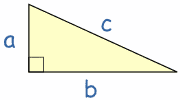
\includegraphics[scale=0.5]{pythagorean.png}}
				\caption{A right triangle. (taken from www.mathsisfun.com)}
				\label{pythagorean}
			\end{figure}
			\begin{equation}
				c^2 = a^2 + b^2
			\end{equation}
			Explain why the Pythagorean Theorem is true.
			
	
\end{document}